\graphicspath{{chapters/02/}}
\chapter{Coverage}
\section{Local Coverage and Allelic Fraction}
Two key concepts needed when perfoming genomics analysis are the \textbf{local coverage} and \textbf{allelic fraction}.

	\paragraph{Local coverage (cov)}
		The local coverage (cov) at position (base) $i$ is the number of reads that span $p_i$.
	\paragraph{Allelic fraction (AF)}
		The allelic fraction (AF) at position $i$ is the proportion of reads that supports 			the reference base in $p_i$, and viceversa. 
		
\subsection{Mapped reads}
The number of mapped reads is always lower than expected. Errors, major translocation that will impair a good mapping of the reads. \\
Difference between physical and sequence coverage. Physical coverage is always higher, and it cheanges if in the assya the PE protocol is used. \\
To put it simply, when calculating the sequence coverage you only take into accountthe actual ends, while when calculating the physical coverage you also acount for the unsequenced part of the PE protocol. 
\begin{figure}[htbp!]
    \centering
    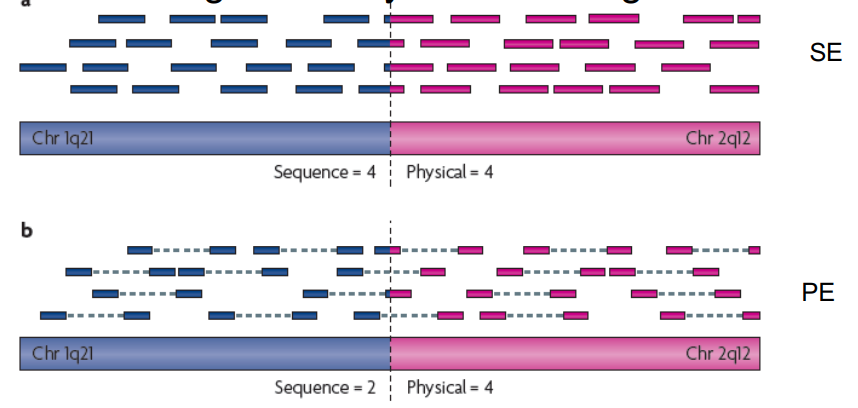
\includegraphics[width=0.5\textwidth]{seq_phys.png}
    \caption{Schematic difference between sequence (on the left) and physical coverage (on the right). From Meyerson et al., Nature Reviews Genetics 2010}
    \label{fig:seq_phys}
\end{figure}Formal definitions are:

\paragraph{Sequence coverage:}
		amount of oversampling (how many times a base is sequenced); to detect nucleotide alterations with high sensitivity, the 3 billion bases of the human genome have typically been ‘covered’ with at least 30-fold (30X) on average, meaning 90 billiion bases of sequence data per sample. 
	\paragraph{Physical coverage:}
		the expected distance between the paired reads is used to uniquely place the reads on the genome; unexpected read pairs are used to detect structural anomalies.

\section{When to increase the intended coverage of a NGS assay}
In some experiments setups there's the need to carefully control the amount of intended coverage. \\
If we are looking for SNPs only, which by definition are present in all of the cells, we only need enough redundacy (local coverage) to detect them and distinguish the reference base and the alternative base (in case of an heterozygous SNP we will ideally find half of the reads supporting the reference and half supporting the alternatice).\\
However, if the sample comes from a tumor or hematopoietic events, we need to look for subclonal events. Subclonal events are not harboured by all of the cells but only by a fraction of them. If we expect 1/4 of the cells harbouring the mutation, we need to increase the coverage. \\
The same reasoning goes for any monozygous mutation and any rare of low abundant events. 

\begin{figure}[htbp!]
    \centering
    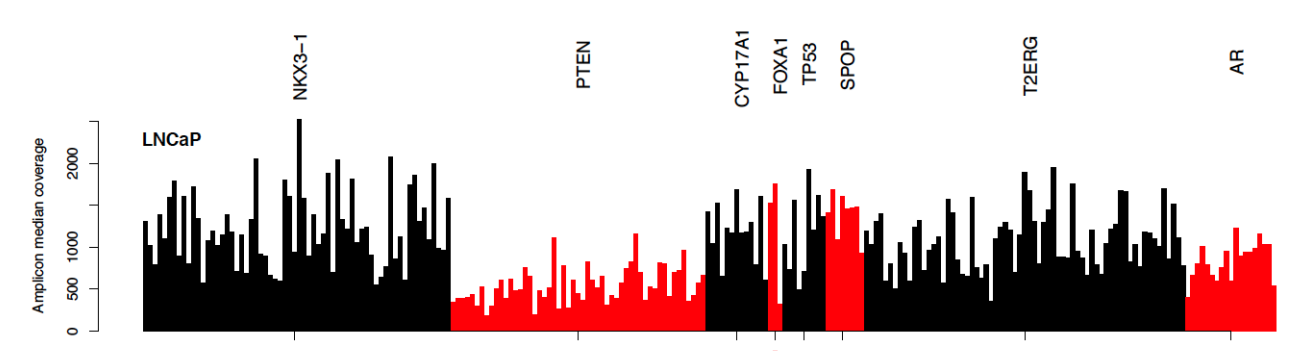
\includegraphics[width=0.5\textwidth]{local_coverage.png}
    \caption{Example of local coverage. On the x axis genomic location (on top e ery gene) and the bars is the number of amplicons. }
    \label{fig:local}
\end{figure}

In figure \ref{fig:local} a barplot can be observed, representing the local coverage (y axis) in the gene locations (x axis). The cov is on average about 600x and it's "wavy", not evenly distributed (very typical). However, if one would do an average of the coverage for each gene, they would discover that one gene is abuntantly underrepresented: PTEN.\\
What's happening on PTEN base on plot \ref{fig:local}? Probably, the most accurate guess is a deletion. But of which kind? For sure not a homozygous deletion, since we would not be able to see any signal in the plot. From this data however we cannot say wether this is a monoallelic or biallelic deletion. \\
Note that this (and the following) plot is the actual way sequencing data is shown, while the figure presented in \ref{SE_PE} was a schematic representation. 

\begin{figure}[htbp!]
    \centering
    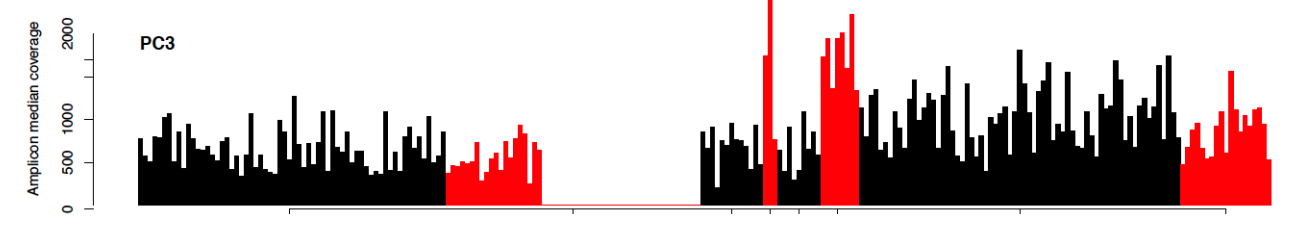
\includegraphics[width=0.5\textwidth]{local_coverage1.png}
    \caption{Example 2 of local coverage. The  cell line is different (PC3 instead of LNCaP). }
    \label{fig:local1}
\end{figure}

However, in the plot \ref{fig:local1}, from a different cell line, we can see a clear monoallelic deletion and a partiall biallelic deletion of PTEN.\\

\begin{figure}[htbp!]
    \centering
    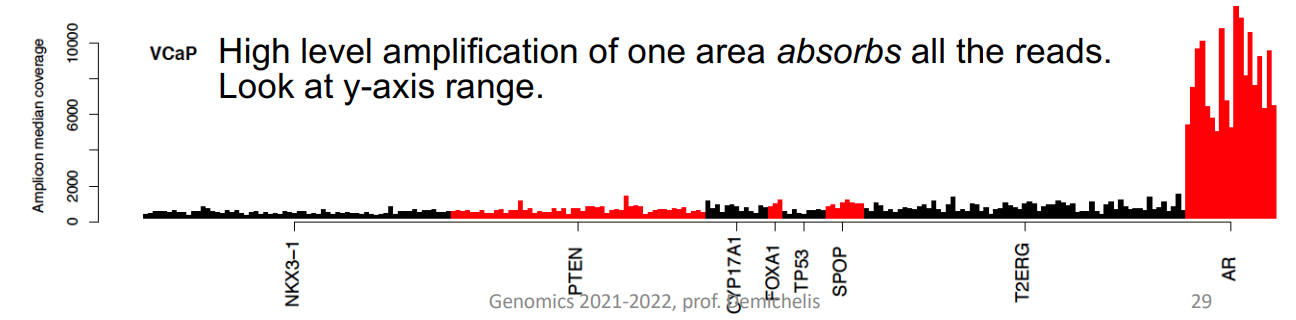
\includegraphics[width=0.5\textwidth]{local_coverage2.png}
    \caption{Example 3 of local coverage. The  cell line is different (VCaP). The massive amplification of the AR region is typicall in advanced prostate cancer.}
    \label{fig:local2}
\end{figure}

In figure \ref{fig:local2} we can see a massive amplification of the antigen receptor. Mistake in the assay: amplification on the AR does not allow the analysis / discovery of other copy number variations because all of the reads will go to the AR site. \\
These were amplicon-based approaches. 
With NGS instead, It is easy to increase the experimental coverage (i.e. the sequence depth) at later point. 
Provided your original sample/library is still available, you can perform another run of sequencing and then combine the output from different runs. 
Note that this isn’t possible with array-based technologies.\\
However, there are some What are the limiting factors of NGS DNA-seq experiments. Problems with repeated regions is one, but also not knowing the linearity of the genome. If the sequencing is done with long reads, there are more errors but allow for sequencing of longer molecules. 

\section{Interpreting Pair Orientations}
Performed using IGV. Its main characteristic is that it's a one window viewer 
\subsection{Inversion}
Reads that span the breakpoint. \\
What's happening exactly at the breakpoint? What's the coverage when looking at the data? Because the sequence that we have in the molecule does not exist there and therefore that sequence doe not exist in two copies in the molecule. 
Drop in local coverage.  
In the target molecule, either does not exist or exist only in one allele and not the other one. \\
Interpreting structural variance: not only orientation but also coverage at the exact break point. 


\begin{figure}[htbp!]
    \centering
    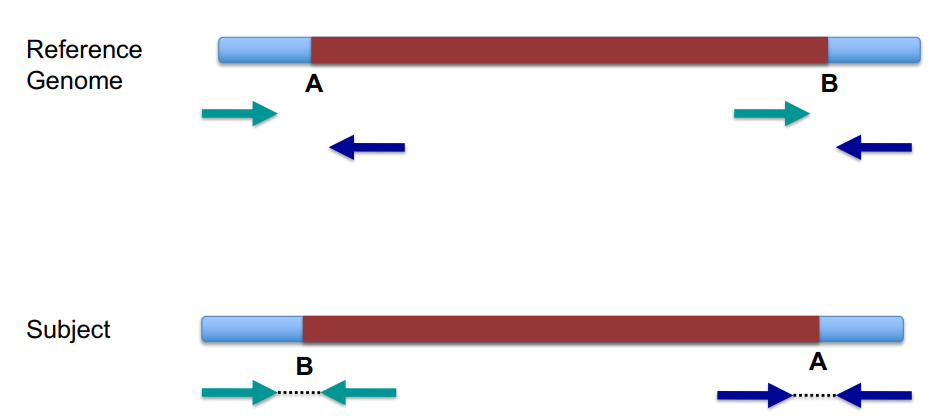
\includegraphics[width=0.5\textwidth]{inversion.png}
    \caption{Inversion disocvering exploiting PE reads.}
    \label{fig:inversion}
\end{figure}


\subsection{Tandem duplication}
Notice how in the tandem dupication all the reads that do not cover the junction point align perfectly to the reference, resulting in doubled coverage.\\
No drop of coverage because the sequences also exist in the reference. \\

\begin{figure}[htbp!]
    \centering
    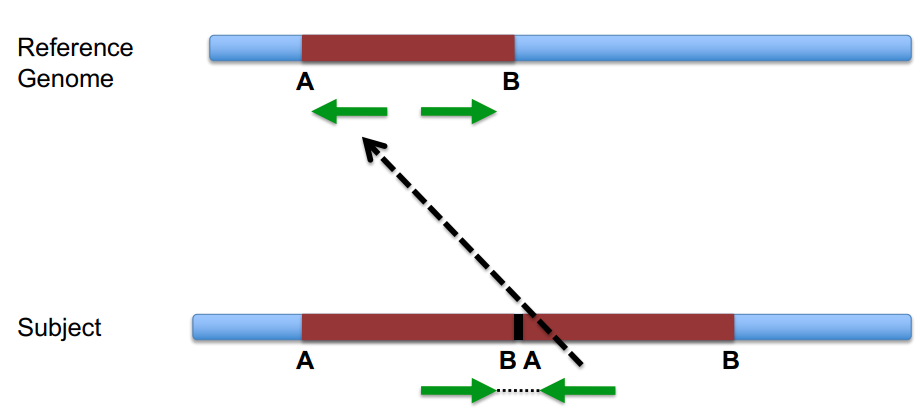
\includegraphics[width=0.5\textwidth]{tandem.png}
    \caption{Tandem duplication discovering exploiting PE reads.}
    \label{fig:inversion}
\end{figure}

\subsection{Inverted duplication}
We expect double coverage in the duplicatd site in the reference genome. 
\begin{figure}[htbp!]
    \centering
    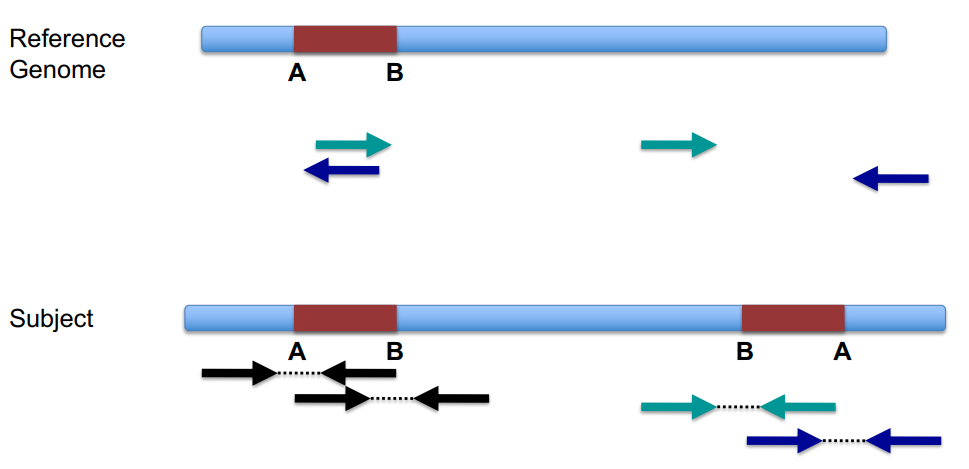
\includegraphics[width=0.5\textwidth]{inverted.png}
    \caption{Inverted duplication discovering exploiting PE reads.}
    \label{fig:inversion}
\end{figure}

What if we have a deletion? How can you guess the size of a deletion? ither you look at the coverage or observed distance between the reads, gives clean indication of the size of the deletion. For tiny deletions, smaller than the length of the read, you use the sequence within the reads and in this way disocvering indels.  

\section{Summary}
















